% Created 2022-11-25 Fri 12:10
% Intended LaTeX compiler: pdflatex
\documentclass[presentation,aspectratio=1610]{beamer}
\usepackage[utf8]{inputenc}
\usepackage[T1]{fontenc}
\usepackage{graphicx}
\usepackage{grffile}
\usepackage{longtable}
\usepackage{wrapfig}
\usepackage{rotating}
\usepackage[normalem]{ulem}
\usepackage{amsmath}
\usepackage{textcomp}
\usepackage{amssymb}
\usepackage{capt-of}
\usepackage{hyperref}
\usepackage{khpreamble, euscript}
\DeclareMathOperator{\atantwo}{atan2}
\newcommand*{\ctrb}{\EuScript{C}}
\newcommand*{\obsv}{\EuScript{O}}
\usetheme{default}
\author{Kjartan Halvorsen}
\date{\today}
\title{Discrete-time Ouput feedback (state feedback with observer)}
\hypersetup{
 pdfauthor={Kjartan Halvorsen},
 pdftitle={Discrete-time Ouput feedback (state feedback with observer)},
 pdfkeywords={},
 pdfsubject={},
 pdfcreator={Emacs 26.3 (Org mode 9.4.6)}, 
 pdflang={English}}
\begin{document}

\maketitle

\section{Discret-time state space model}
\label{sec:orgcce3085}
\begin{frame}[label={sec:orga03e75f}]{The discrete-time state-space model}
\end{frame}

\begin{frame}[label={sec:org1b7eb53}]{The discrete-time state-space model}
\begin{center}
  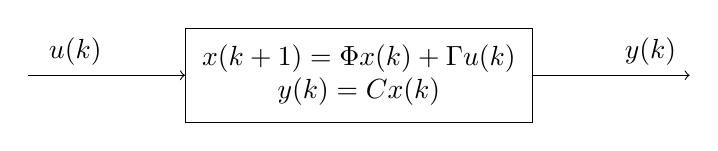
\begin{tikzpicture}[node distance=42mm, block/.style={inner sep=6pt, rectangle, draw, minimum width=15mm}, sumnode/.style={circle, draw, inner sep=2pt}]
    \node[coordinate] (input) {};
    \node[block, right of=input, align=center] (plant)  {$x(k+1) = \Phi x(k) + \Gamma u(k)$\\$y(k) = C x(k)$};
    \node[coordinate, right of=plant] (output) {};

    \draw[->] (input) -- node[above, pos=0.3] {$u(k)$} (plant);
    \draw[->] (plant) -- node[above, near end] {$y(k)$} (output);
  \end{tikzpicture}
\end{center}
\end{frame}


\begin{frame}[label={sec:org5d3c8a5}]{Stability}
\end{frame}
\begin{frame}[label={sec:org97893af}]{Eigenvalues and eigenvectors}
\alert{Definition} The eigenvalues \(\lambda_i  \in \mathbb{R}\) and eigenvectors \(v_i \in \mathbb{R}^n\) of a matrix \(\Phi \in \mathbb{R}^{n\times{}n}\) are the \(n\) pairs \((\lambda_i, v_i \neq 0 ), \; i=1,2,\ldots,n\) that satisfy
\[ \Phi v_i = \lambda_i v_i \]
\end{frame}

\begin{frame}[label={sec:org97f83c4}]{Stability}
The system
\begin{equation*}
x(k+1)=\Phi x(k), \ \ x(0)=x_0
\end{equation*}
is \alert{stable} if  \(\underset{t\to\infty}{\lim}x(kh)=0, \quad \forall\;  x_0\in\Bbb{R}^n\).

A necessary and sufficient requirement for stability is that \alert{all the eigenvalues of \(\Phi\) are inside the unit circle.}

The \alert{eigenvalues} of \(\Phi\) are the  \alert{poles} of the system.
\end{frame}

\section{State feedback}
\label{sec:org22f7393}
\begin{frame}[label={sec:orgc1d1c16}]{State feedback control}
\end{frame}
\begin{frame}[label={sec:org7e36995}]{State feedback control}
Given
 \begin{equation}
 \begin{split}
  x(k+1) &= \Phi x(k) + \Gamma u(k)\\
  y(k) &= C x(k)
 \end{split}
 \label{eq:ssmodel}
\end{equation}
and measurements (or an estimate) of the state vector \(x(k)\). 

\alert{Linear state feedback} is the control law
\begin{equation*}
\begin{split}
 u(k) &= f\big((x(k), u_c(k)\big) = -\textcolor{morange}{l_1}x_1(k) - \textcolor{morange}{l_2}x_2(k) - \cdots - \textcolor{morange}{l_n} x_n(k) + \textcolor{mbluegreen}{l_0}u_c(k)\\
      &= -\textcolor{morange}{L}x(k) + \textcolor{mbluegreen}{l_0}u_c(k), 
\end{split}
\end{equation*}
where \[ \textcolor{morange}{L} = \bbm \textcolor{morange}{l_1} & \textcolor{morange}{l_2} & \cdots & \textcolor{morange}{l_n} \ebm. \]
Substituting this in the state-space model \eqref{eq:ssmodel} gives
 \begin{equation}
 \begin{split}
  x(k+1) &= \left(\Phi -\Gamma \textcolor{morange}{L} \right) x(k) + \textcolor{mbluegreen}{l_0}\Gamma u_c(k)\\
  y(k) &= C x(k)
 \end{split}
 \label{eq:closedloop}
\end{equation}
\end{frame}

\begin{frame}[label={sec:org9b791d2}]{Pole placement by state feedback}
Given (or choosing) a desired placement of the closed-loop poles \(p_1, p_2, \ldots, p_n\), being roots of the desired characteristic polynomial
\begin{equation}
a_c(z) = (z-p_1)(z-p_2)\cdots(z-p_n) = z^n + \alpha_1 z^{n-1} + \cdots \alpha_n.
\label{eq:desiredpoles}
\end{equation}

\pause

Linear state feedback gives the system
 \begin{equation}
 \begin{split}
  x(k+1) &= \left(\Phi -\Gamma \textcolor{morange}{L} \right) x(k) + \textcolor{mbluegreen}{l_0}\Gamma u_c(k)
 \end{split}
 \label{eq:closedloop}
\end{equation}
with characteristic polynomial
\begin{equation}
\det\left(zI - (\Phi - \Gamma \textcolor{morange}{L})\right) = z^n + \beta_1(\textcolor{morange}{l_1},\ldots,\textcolor{morange}{l_n}) z^{n-1} + \cdots \beta_n(\textcolor{morange}{l_1}, \ldots, \textcolor{morange}{l_n}).
\label{eq:poles}
\end{equation}

\pause

Set the coefficients of the desired characteristic polynomial \eqref{eq:desiredpoles} equal to the coefficients of \eqref{eq:poles} to obtain the system of equations
\begin{equation*}
\begin{split}
\beta_1(\textcolor{morange}{l_1}, \ldots, \textcolor{morange}{l_n}) &= \alpha_1\\
\beta_2(\textcolor{morange}{l_1}, \ldots, \textcolor{morange}{l_n}) &= \alpha_2\\
&\vdots\\
\beta_n(\textcolor{morange}{l_1}, \ldots, \textcolor{morange}{l_n}) &= \alpha_n
\end{split}
\label{eq:coeffs}
\end{equation*}
\end{frame}

\begin{frame}[label={sec:orgd5bbdf5}]{Pole placement by state feedback}
The system of equations
\begin{equation*}
\begin{split}
\beta_1(\textcolor{morange}{l_1}, \ldots, \textcolor{morange}{l_n}) &= \alpha_1\\
\beta_2(\textcolor{morange}{l_1}, \ldots, \textcolor{morange}{l_n}) &= \alpha_2\\
&\vdots\\
\beta_n(\textcolor{morange}{l_1}, \ldots, \textcolor{morange}{l_n}) &= \alpha_n
\end{split}
\label{eq:coeffs}
\end{equation*}

is always linear in the parameters of the controller, hence
\begin{equation*}
M \textcolor{morange}{L}\transp = \alpha,
\end{equation*}
where \(\alpha\transp = \bbm \alpha_1 & \alpha_2 & \cdots & \alpha_n \ebm.\)
\end{frame}

\begin{frame}[label={sec:org1c526d4},fragile]{Pole placement by state feedback}
 Given a desired placement of the closed-loop poles \(p_1, p_2, \ldots, p_n\), being roots of the desired characteristic polynomial
\begin{equation*}
a_c(z) = (z-p_1)(z-p_2)\cdots(z-p_n) = z^n + \alpha_1 z^{n-1} + \cdots \alpha_n.
\label{eq:desiredpoles}
\end{equation*}
and closed-loop system
 \begin{equation*}
 \begin{split}
  x(k+1) &= \left(\Phi -\Gamma \textcolor{morange}{L} \right) x(k) + \textcolor{mbluegreen}{l_0}\Gamma u_c(k)\\
  y(k) &= C x(k)
 \end{split}
 \label{eq:closedloop}
\end{equation*}

The Matlab (\emph{control systems toolbox}) has methods for computing the gain vector \(L\)

\begin{enumerate}
\item \alert{Ackerman's method} 
\begin{verbatim}
L = acker(Phi, Gamma, pd)
\end{verbatim}
\item \alert{Numerically more stable method} 
\begin{verbatim}
L = place(Phi, Gamma, pd)
\end{verbatim}
\end{enumerate}
\end{frame}

\begin{frame}[label={sec:org98b4743}]{The reference input gain \(l_0\)}
The closed-loop state space system
\begin{equation*}
\begin{split}
 x(k+1) &= \underbrace{\left(\Phi -\Gamma \textcolor{morange}{L} \right)}_{\Phi_c} x(k) + \textcolor{mbluegreen}{l_0}\Gamma u_c(k)\\
 y(k) &= C x(k)
\end{split}
\end{equation*}
with constant reference signal \(u_c(k) = u_{c,f}\) has the steady-state solution (\(x(k+1)=x(k)\))
\pause
\[ x_f =  \textcolor{mbluegreen}{l_0} (I - \Phi_c)^{-1}\Gamma u_{c,f}\]
\[ y_f = Cx_f = \textcolor{mbluegreen}{l_0} C(I - \Phi_c)^{-1}\Gamma u_{c,f}.\]
We want \(y_f =  u_{c,f}\),
\[ \Rightarrow \qquad \textcolor{mbluegreen}{l_0} = \frac{1}{C(I-\Phi_c)^{-1}\Gamma}\]
\end{frame}

\section{State feedback with observer}
\label{sec:org4879af8}
\begin{frame}[label={sec:org7fa7c18}]{State feedback with reconstructed states}
\end{frame}

\begin{frame}[label={sec:orgb008220}]{Observer design}
Given model
 \begin{equation*}
 \begin{split}
  x(k+1) &= \Phi x(k) + \Gamma u(k)\\
  y(k) &= C x(k)
 \end{split}
 \label{eq:ssmodel}
\end{equation*}
and measurements of the output signal \(y(k)\). 

The observer is given by
\begin{equation*}
\begin{split}
\hat{x}(k+1) &= \underbrace{\Phi \hat{x}(k) + \Gamma u(k)}_{\text{simulation}} + \underbrace{\textcolor{mred}{K}\big(y(k) - C\hat{x}(k)\big)}_{\text{correction}} = \left(\Phi - \textcolor{mred}{K}C\right)\hat{x}(k) +  \Gamma u(k) + \textcolor{mred}{K}y(k)
\end{split}
\end{equation*}
with poles given by the eigenvalues of the matrix \(\Phi_o = \Phi - \textcolor{mred}{K}C\)

\alert{Rule-of-thumb} (From continous-time state-space theory) Choose the poles of the observer (eigenvalues of \(\Phi-\textcolor{mred}{K}C\)) at least twice as fast as the poles (eigenvalues) of \(\Phi-\Gamma L\). In discrete-time place the observer-poles closer to the origin.  
\end{frame}


\begin{frame}[label={sec:org7bf85df}]{Control by feedback from reconstructed states}
The design problem can be separates into two problems
\begin{enumerate}
\item Determine the gain vector \(\textcolor{orange!80!black}{L}\) and the gain \(l_0\) of the control law
\[ u(k) = -\textcolor{orange!80!black}{L} \hat{x}(k) + l_0 u_c(k)\]
so that the closed-loop system has good reference tracking.
\item Determine the gain vector \(\textcolor{mred}{K}\) of the observer
\begin{equation*}
\begin{split}
\hat{x}(k+1) &= \Phi \hat{x}(k) + \Gamma u(k) + \textcolor{mred}{K} \big(y(k) - C\hat{x}(k)\big)
\end{split}
\end{equation*}
to get a good balance between disturbance rejection and noise attenuation.
\end{enumerate}
\end{frame}

\begin{frame}[label={sec:org7c6078e}]{Computing the observer gain}
A matrix \(M\) and its transpose \(M\transp\) have the same eigenvalues. Hence, the problem of determining the gain \(K\) to obtain desired eigenvalues of 
\[\Phi- \textcolor{mred}{K}C\] is equivalent to determining the gain \(K\) in 
\[(\Phi-KC)\transp = \Phi\transp - C\transp \textcolor{mred}{K}\transp.\]
The last problem has the exact same form as the problem of determining \(L\) to obtain desired eigenvalues of 
\[\Phi - \Gamma L\]

So, the same matlab function can be used for both problems.
\end{frame}

\begin{frame}[label={sec:org2df0796},fragile]{Computing the observer gain}
 \begin{enumerate}
\item \alert{Ackerman's method} 
\begin{verbatim}
K = acker(Phi', C', po)'
\end{verbatim}
\item \alert{More numerically stable method} 
\begin{verbatim}
K = place(Phi', C', pd)'
\end{verbatim}
\end{enumerate}
\end{frame}



\section{Where to choose the poles}
\label{sec:org5d05aaa}
\begin{frame}[label={sec:org93e0678}]{Where to place the closed-loop poles?}
\end{frame}
\begin{frame}[label={sec:org0ab5382}]{Where to place the closed-loop poles?}
If the system is controllable we can place the closed-loop poles freely.

\pause

But not all placements are good choices

\pause

Take into account
\begin{itemize}
\item Desired speed
\item Desired damping
\item \alert{Poles and zeros of the plant}
\end{itemize}
\end{frame}

\begin{frame}[label={sec:org77b05b0}]{Placing for desired speed and damping}
\begin{columns}
\begin{column}{0.4\columnwidth}
\alert{s-plane}

\begin{center}
 \includegraphics[height=.6\textheight]{../../figures/sgrid-crop}
\end{center}
\end{column}
\begin{column}{0.6\columnwidth}
\alert{z-plane}
\begin{center}
 \includegraphics[height=.59\textheight]{../../figures/zgrid-crop}
\end{center}
\end{column}
\end{columns}
\end{frame}

\begin{frame}[label={sec:org6b19ed2}]{The effect of plant zeros and poles}
\begin{columns}
\begin{column}{0.4\columnwidth}
\begin{center}
 \includegraphics[width=1.0\linewidth]{../../figures/AM-portal.png}
\end{center}

\pause
\end{column}

\begin{column}{0.6\columnwidth}
\begin{center}
 \includegraphics[width=1.0\linewidth]{../../figures/AM-ch12.4.png}
\end{center}
\end{column}
\end{columns}
\end{frame}


\begin{frame}[label={sec:orga0e6da5}]{Placing w.r.t plant zeros and poles}
\begin{itemize}
\item Cancel slow plant zeros
\item Place fast closed-loop poles near fast plant poles
\end{itemize}
\end{frame}
\end{document}